\RequirePackage[l2tabu, orthodox]{nag}

\documentclass[10pt]{scrartcl}
\usepackage[T1]{fontenc}
\usepackage{amsmath,amsfonts,amssymb}
\usepackage{mathtools}
\usepackage{cancel}
\usepackage[usenames,dvipsnames]{color}
\usepackage{soul}
\usepackage[margin=2cm,letterpaper]{geometry}
\usepackage{enumerate}
\usepackage{graphicx}
\usepackage[colorlinks=true,urlcolor=blue]{hyperref}
\usepackage{floatrow}
\usepackage{deluxetable}
\usepackage{verbatim}
\usepackage{fancyvrb}
\usepackage{listings}
\usepackage{calc}
\usepackage{xfrac}
\usepackage{cleveref}
\usepackage[font=small]{caption}
\usepackage[font=scriptsize]{subcaption}
\usepackage[activate={true,nocompatibility},final,tracking=true,kerning=true,spacing=true,factor=1100,stretch=10,shrink=10]{microtype}

\SetTracking{encoding={*}, shape=sc}{40}

\microtypecontext{spacing=nonfrench}

\floatsetup{ 
  heightadjust=object,
  valign=t
}

\definecolor{Light}{gray}{.90}
\sethlcolor{Light}

\newcommand{\code}[1]{\hl{\texttt{#1}}}

\lstset{%
language=IDL,                   % choose the language of the code
basicstyle=\footnotesize\sffamily,%\ttfamily\footnotesize,       % the size of the fonts that are used for the code
commentstyle=\color{red},
numbers=left,                   % where to put the line-numbers
numberstyle=\footnotesize,      % the size of the fonts that are used for the line-numbers
stepnumber=1,                   % the step between two line-numbers. If it is 1 each line will be numbered
numbersep=5pt,                  % how far the line-numbers are from the code
showspaces=false,               % show spaces adding particular underscores
showstringspaces=false,         % underline spaces within strings
showtabs=false,                 % show tabs within strings adding particular underscores
% frame=single,                   % adds a frame around the code
backgroundcolor=\color{Light},
columns=flexible,
tabsize=2,                      % sets default tabsize to 2 spaces
captionpos=b,                   % sets the caption-position to bottom
breaklines=true,                % sets automatic line breaking
breakatwhitespace=true,        % sets if automatic breaks should only happen at whitespace
escapechar={\%*},          % if you want to add a comment within your code
morecomment=[l][\color{OliveGreen}]{**},
}

\title{Everything You Need to Know to Run The Most Recent Program}
\author{Jeren Suzuki}
\date{Last Edited \today}

\begin{document}

\pagenumbering{gobble}
\maketitle
\tableofcontents
\addcontentsline{toc}{section}{Introduction}
\clearpage
\pagenumbering{arabic}

\section*{Introduction}
\label{sec:introduction}
If you read this document, you will understand what the commands/outputs are for the most recent sun centering program. That's it.
% section introduction (end)

\section{Main Program} % (fold)
\label{sec:main_program}
The main program is called \code{alpha.pro} and spits out images in X11 windows and center positions in the terminal window. 


Content of \code{alpha.pro} with coded in comments defined by lines starting with `;' and my comments within the \LaTeX{} document starting with `**':

\begin{lstlisting}[texcl=false]
; docformat = 'rst'
PRO alpha
;+
;   :Description:
;      Finds the center of N whole suns and M partial suns using limb-fitting for the whole suns and simple centroiding for the partial suns
;
;   :Params:
;
;   :TODO: 
;       NONE, BRAH
;
; idldoc,root='../suncentering', output='rbdoc',format_style='rst',/user,/quiet,markup_style='rst'
;-
**
** The command above produces html documentation on all the .pro files starting from the main directory and branching into all sub-directories with the %*\href{http://idldoc.idldev.com/}{IDLdoc}%* program. The document markup syntax is reStructuredText, otherwise known as %*\href{http://docutils.sourceforge.net/rst.html}{rst}%*.
**

COMPILE_OPT idl2

; Our list of images to take centers of
wholeimage  = MRDFITS('../fits_files/dottedimage.fits',/sil) 
w1_w2_p3    = MRDFITS('../fits_files/partial3rd.fits',/sil)
w1_p2_p3    = MRDFITS('../fits_files/2partials.fits',/sil)
reg12       = MRDFITS('../fits_files/1_2.fits',/sil)
reg13       = MRDFITS('../fits_files/1_3.fits',/sil)
reg23       = MRDFITS('../fits_files/2_3.fits',/sil)
w2_p3       = MRDFITS('../fits_files/w2_p3.fits',/sil)
p1_w2_w3    = MRDFITS('../fits_files/p1_w2_w3.fits',/sil)
p1_w2_p3    = MRDFITS('../fits_files/p1_w2_p3.fits',/sil)
p1_p2_w3    = MRDFITS('../fits_files/p1_p2_w3.fits',/sil)
w1_p2_w3    = MRDFITS('../fits_files/w1_p2_w3.fits',/sil)
p1_w3       = MRDFITS('../fits_files/p1_w3.fits',/sil)
p1_w2       = MRDFITS('../fits_files/p1_w2.fits',/sil)
w1_p3       = MRDFITS('../fits_files/w1_p3.fits',/sil)
brightsun   = MRDFITS('../fits_files/albsun.fits',/sil)
corner      = MRDFITS('../fits_files/corner.fits',/sil)
corner2     = MRDFITS('../fits_files/corner2.fits',/sil)
corner3     = MRDFITS('../fits_files/corner3.fits',/sil)
dimsun      = MRDFITS('../fits_files/sun2.fits',/sil)
tritest     = MRDFITS('../fits_files/tritest.fits',/sil)

**
** Each of these fits files is a byte image of a sun or multiple suns
**

; Toggling which image is going to be analyzed

startimage=wholeimage
; startimage=w1_w2_p3
; startimage=w1_p2_p3
; startimage=reg12
; startimage=reg23
; startimage=reg13
; startimage=w2_p3
; startimage=p1_w2_w3
; startimage=p1_w2_p3
; startimage=p1_p2_w3
; startimage=w1_p2_w3
; startimage=p1_w3
; startimage=p1_w2
; startimage=w1_p3
; startimage=brightsun   ;no param list for this one
startimage = dimsun
startimage = tritest

; profiler
; profiler,/system
**
** We only used this when we were benchmarking the program for speed. As it is now, it should be fast enough.
**
; takes ~.07 s to run albert's triple sun image


tic
defparams, 'pblock_albtritest.txt'
; defparams, 'pblock_albdimsun.txt'
; defparams, 'pblock_orig_small.txt'
** Here we load the parameter *.txt file and store all the variables into a global variable, !param **
toc
; .0005 to here
defsysvarthresh, startimage
** 
**  With the variables just defined, we load the starting image, sort the 2D image into a 1D arary, chop off the top .1% pixels, then take the 2nd derivative and calculate thresholds. defsysvarthresh calls %*\code{idsuns}%* and %*\code{setbetterpeak}%*
**
toc
; .03 to here
grannysmith = everysun(startimage)
**
** With the thresholds defined from defsysvarthresh, we centroid whatever suns are in the image, regardless if they are in a bad position in the image. 
**
toc
; .065 to here
fuji = picksun_rot(startimage, grannysmith)
**
** Now we look at each solar center and make sure it's not too close to the edge of the image or the bottom corners.
**
toc
; .065 to here
limbfittedcentroids=centroidwholesuns(fuji,startimage)
**
** With a list of ``good'' suns, we crop a box around the centers, making sure not to cut off any part of the sun. Then, we take 5 slices in each direction centered around the solar center. The locations of these chords that cross the limbs of the sun are fitted with a polynomial. Then, we take the midpoint of each chord bounded by where the polynomail crosses the threshold. We average the midpoints and get a limb-fitted center position. 
**
toc
; .068 to here
bbb = para_fid(startimage,limbfittedcentroids)
**
** Now, with the limb-fitted center, we look analyze the sun for fiducials. 
**
; .07 to here
toc
tmpimage = startimage

if N_ELEMENTS(limbfittedcentroids) gt 1 then begin
    for i =0,N_ELEMENTS(limbfittedcentroids)-1 do begin
        tmpimage[limbfittedcentroids[i].limbxpos-1:limbfittedcentroids[i].limbxpos+1,*] = 255
        tmpimage[*,limbfittedcentroids[i].limbypos-1:limbfittedcentroids[i].limbypos+1] = 255
    endfor
endif else begin
    tmpimage[limbfittedcentroids[0].limbxpos-1:limbfittedcentroids[0].limbxpos+1,*] = 255
    tmpimage[*,limbfittedcentroids[0].limbypos-1:limbfittedcentroids[0].limbypos+1] = 255
endelse

**
** Here, we draw lines in the starting image corresponding to the X and Y positions of each sun.
**

; so the rough center is a bit off. Gasp! Why though?

; profiler,/report,data=data
; profiler,/reset,/clear
; print,data[sort(-data.time)],format='(A-20, I7, F12.5, F10.5, I9)'

**
** The format above is just so that we can see which use/IDL functions are taking up the most time so we can optimize our code
**

atmp = startimage

; So I have to highlight fiducials

for i = 0,N_ELEMENTS(bbb)-1 do begin
    for j = 0,N_ELEMENTS((*(bbb[i])).fidarr)-1 do begin

        if ((*(bbb[i])).fidarr)[j].subx ne 0 or ((*(bbb[i])).fidarr)[j].suby ne 0 then begin
        atmp[((*(bbb[i])).fidarr)[j].subx + limbfittedcentroids[i].limbxpos - !param.crop_box -1:((*(bbb[i])).fidarr)[j].subx + limbfittedcentroids[i].limbxpos - !param.crop_box+1,((*(bbb[i])).fidarr)[j].suby + limbfittedcentroids[i].limbypos - !param.crop_box-1:((*(bbb[i])).fidarr)[j].suby + limbfittedcentroids[i].limbypos - !param.crop_box+1]=255
        endif
    endfor
endfor

**
** This for loop goes through each fiducial position and marks them white on the starting image
**

; print,'Main sun x pos:',limbfittedcentroids[0].limbxpos
; print,'Main sun y pos:',limbfittedcentroids[0].limbypos
; print,'50% sun x pos: ',limbfittedcentroids[1].limbxpos
; print,'50% sun y pos: ',limbfittedcentroids[1].limbypos
; print,'25% sun x pos: ',limbfittedcentroids[2].limbxpos
; print,'25% sun y pos: ',limbfittedcentroids[2].limbypos

window,0
cgimage,tmpimage,/k
window,1
cgimage,atmp,/k

ztmp = startimage
tic
best4 = best4(limbfittedcentroids,bbb)
**
** With the fiducial positions we calculated, we only care about the 4 closest to the solar center.
**
toc

for i = 0,n_elements(best4)-1 do begin
    for j = 0,n_elements(best4[i].fidarr)-1 do begin
        ztmp[best4[i].fidarr[j].subx + limbfittedcentroids[i].limbxpos - !param.crop_box -1:best4[i].fidarr[j].subx + limbfittedcentroids[i].limbxpos - !param.crop_box+1,$
            best4[i].fidarr[j].suby + limbfittedcentroids[i].limbypos - !param.crop_box-1:$
            best4[i].fidarr[j].suby + limbfittedcentroids[i].limbypos - !param.crop_box+1]=255
    endfor
endfor

**
** Now, we highlight the best 4 fiducials for each sun 
**
window,2
cgimage,ztmp,/k


print,'Brightest sun center position: ',limbfittedcentroids[0].limbxpos,limbfittedcentroids[0].limbypos
print,'50% sun center position: ',limbfittedcentroids[1].limbxpos,limbfittedcentroids[1].limbypos
print,'25% sun center position: ',limbfittedcentroids[2].limbxpos,limbfittedcentroids[2].limbypos


stop
idedfids = idfids(best4)



; What's going on here?

; cgimage,startimage[limbfittedcentroids[0].limbxpos- !param.crop_box:limbfittedcentroids[0].limbxpos+ !param.crop_box,limbfittedcentroids[0].limbypos- !param.crop_box:limbfittedcentroids[0].limbypos+ !param.crop_box],output='tritest_reg1.eps',/k,/display
; cgimage,startimage[limbfittedcentroids[1].limbxpos- !param.crop_box:limbfittedcentroids[1].limbxpos+ !param.crop_box,limbfittedcentroids[1].limbypos- !param.crop_box:limbfittedcentroids[1].limbypos+ !param.crop_box],output='tritest_reg2.eps',/k,/display
; cgimage,startimage[limbfittedcentroids[2].limbxpos- !param.crop_box:limbfittedcentroids[2].limbxpos+ !param.crop_box,limbfittedcentroids[2].limbypos- !param.crop_box:limbfittedcentroids[2].limbypos+ !param.crop_box],output='tritest_reg3.eps',/k,/display

; aa = startimage

; aa[*,limbfittedcentroids[0].limbypos -20]=255
; aa[*,limbfittedcentroids[0].limbypos -10]=255
; aa[*,limbfittedcentroids[0].limbypos]=255
; aa[*,limbfittedcentroids[0].limbypos +10]=255
; aa[*,limbfittedcentroids[0].limbypos +20]=255

; aa = aa[limbfittedcentroids[0].limbxpos- !param.crop_box:limbfittedcentroids[0].limbxpos+ !param.crop_box,limbfittedcentroids[0].limbypos- !param.crop_box:limbfittedcentroids[0].limbypos+ !param.crop_box]
; cgimage,aa,/k,/display,output='5chords.eps'

stop

end
\end{lstlisting}
% section main_program (end)

After running \code{alpha.pro}, 3 images should be outputted:

\begin{figure}[!ht]
\centering
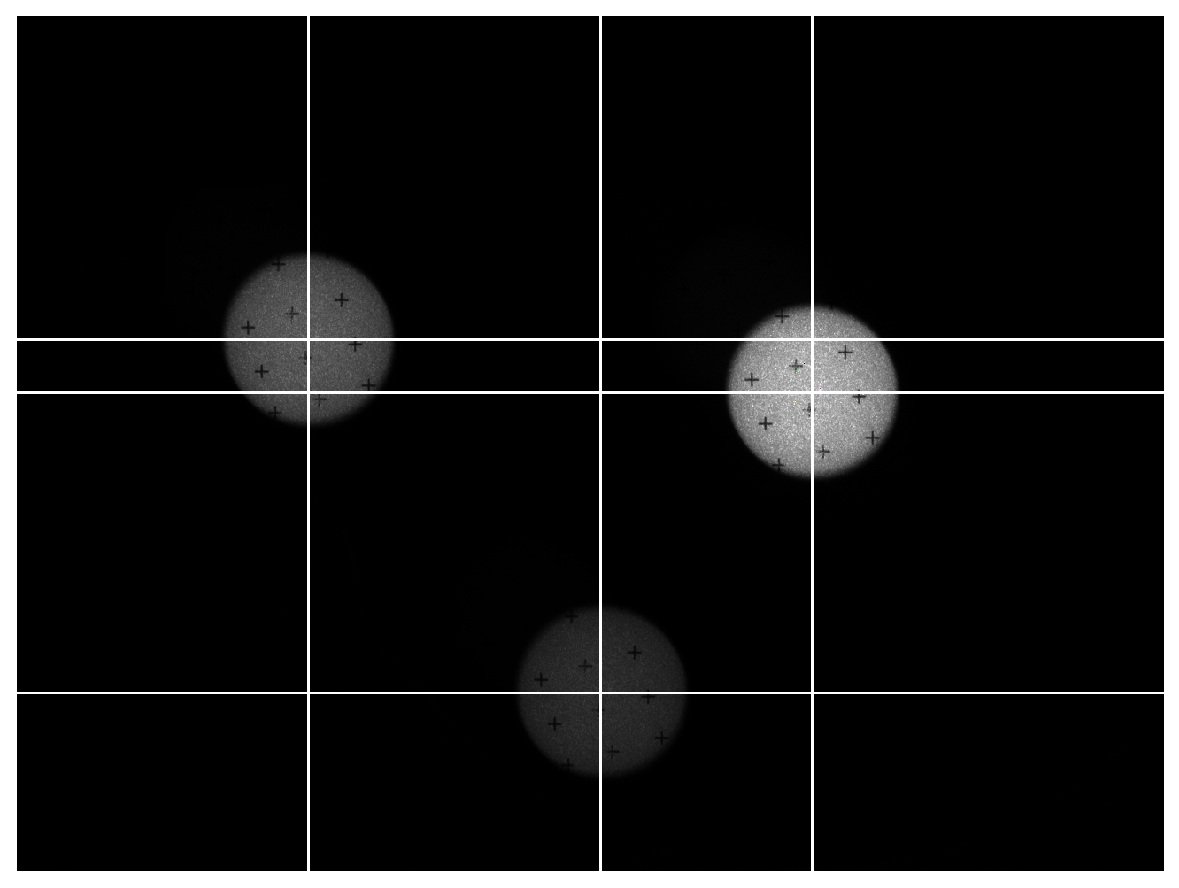
\includegraphics[width=\textwidth]{../plots_tables_images/linecenters.eps}
\caption{Starting image with center positions marked as white lines}
\end{figure}

\begin{figure}[!ht]
    \ffigbox[][\FBheight]{%
    \begin{subfloatrow}[2]%
        \ffigbox[\FBwidth]%
       {%
       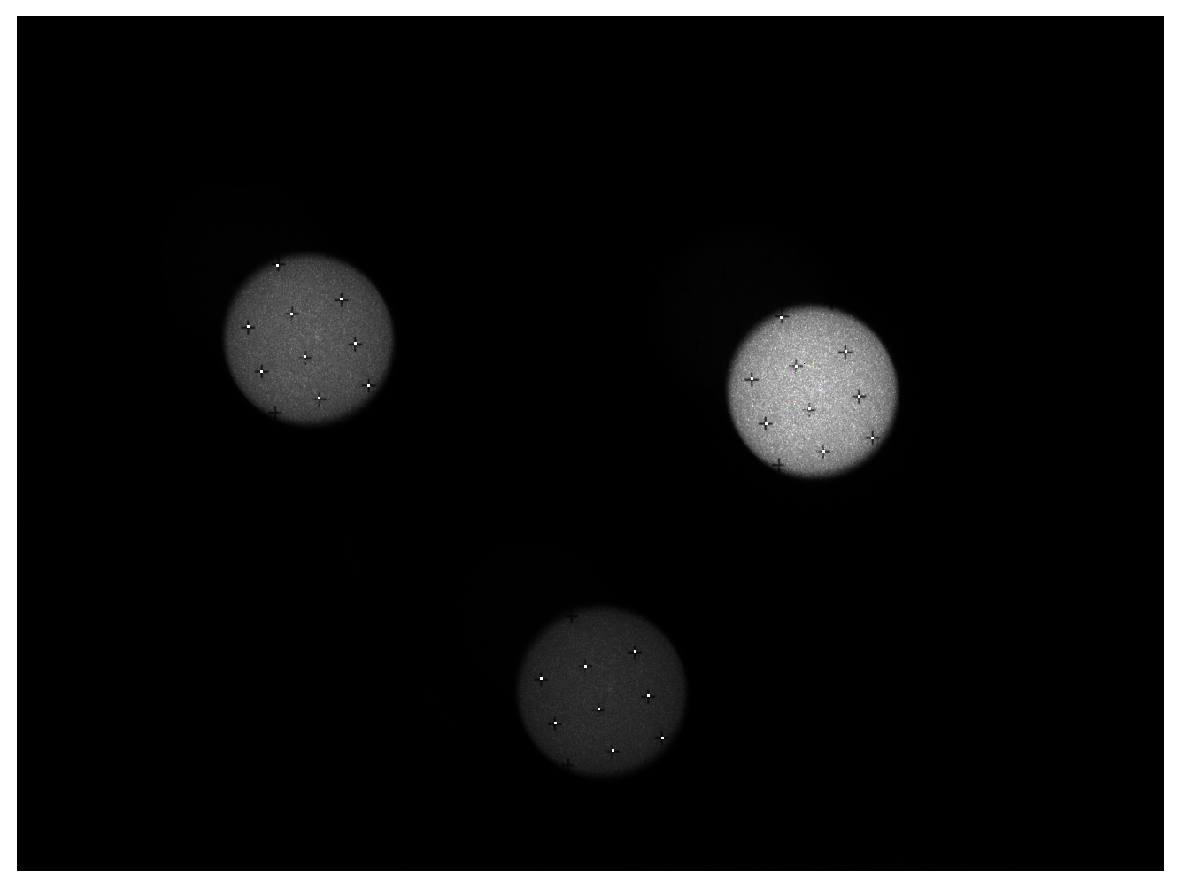
\includegraphics[width=.5\textwidth]{../plots_tables_images/fidpositions.eps}%
       }%
       {%
       \caption{All good fiducials are marked in white}%
       }%
        \ffigbox[\Xhsize]%
       {%
       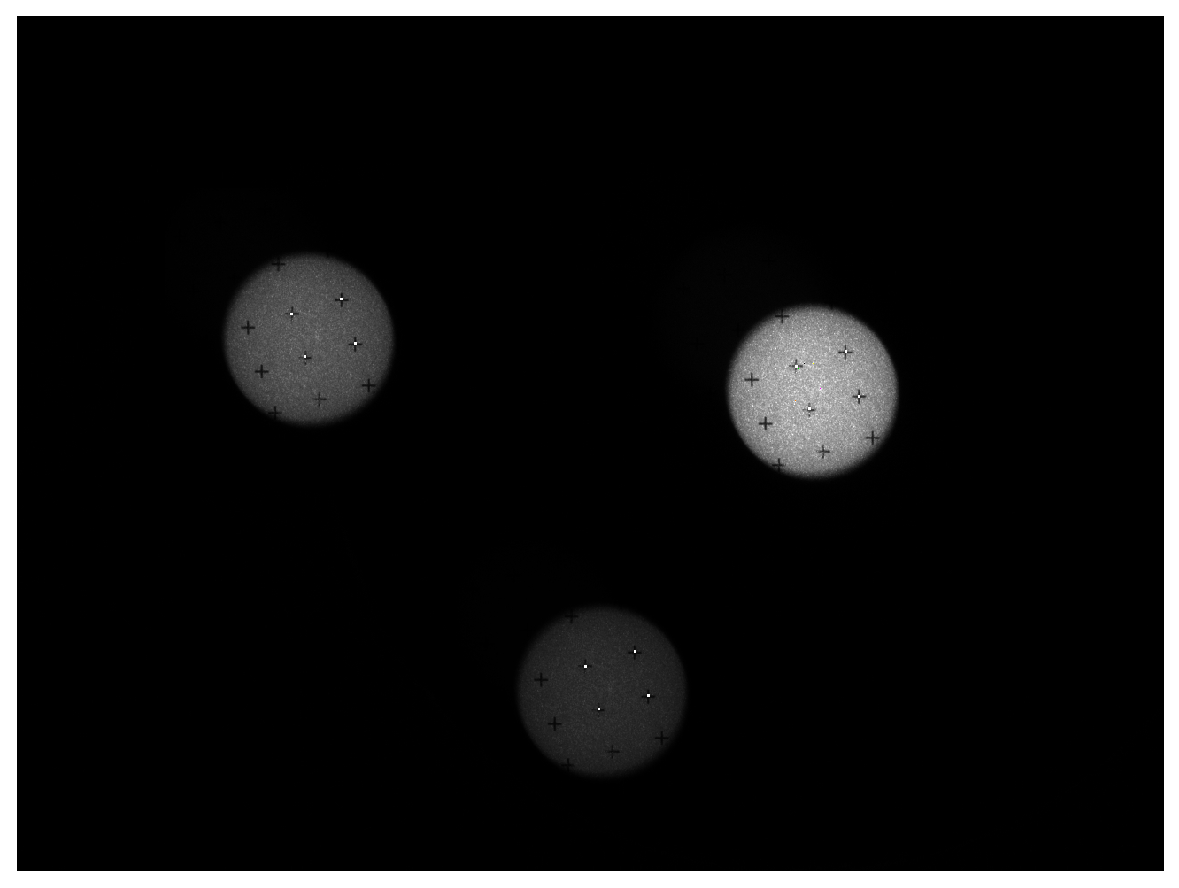
\includegraphics[width=.5\textwidth]{../plots_tables_images/best4fiducials.eps}%
       }%
       {%
       \caption{Only the best 4 fiducials per sun have been marked}%
       }%
    \end{subfloatrow}}{\caption{}\label{alphaoutput}}%
\end{figure}


\end{document}